\documentclass{article}

\usepackage{graphicx}
\usepackage{tikz}
\usepackage{tikzsymbols}
\usetikzlibrary{calc,patterns,shapes.geometric}
\pagestyle{empty}
\usepackage[margin=0pt]{geometry}
\geometry{papersize={14in,12in}}

\def\centerarc[#1](#2)(#3:#4:#5){\draw[#1] ($(#2)+({#5*cos(#3)},{#5*sin(#3)})$) arc (#3:#4:#5);}

\begin{document}
	\begin{figure}
		\centering
		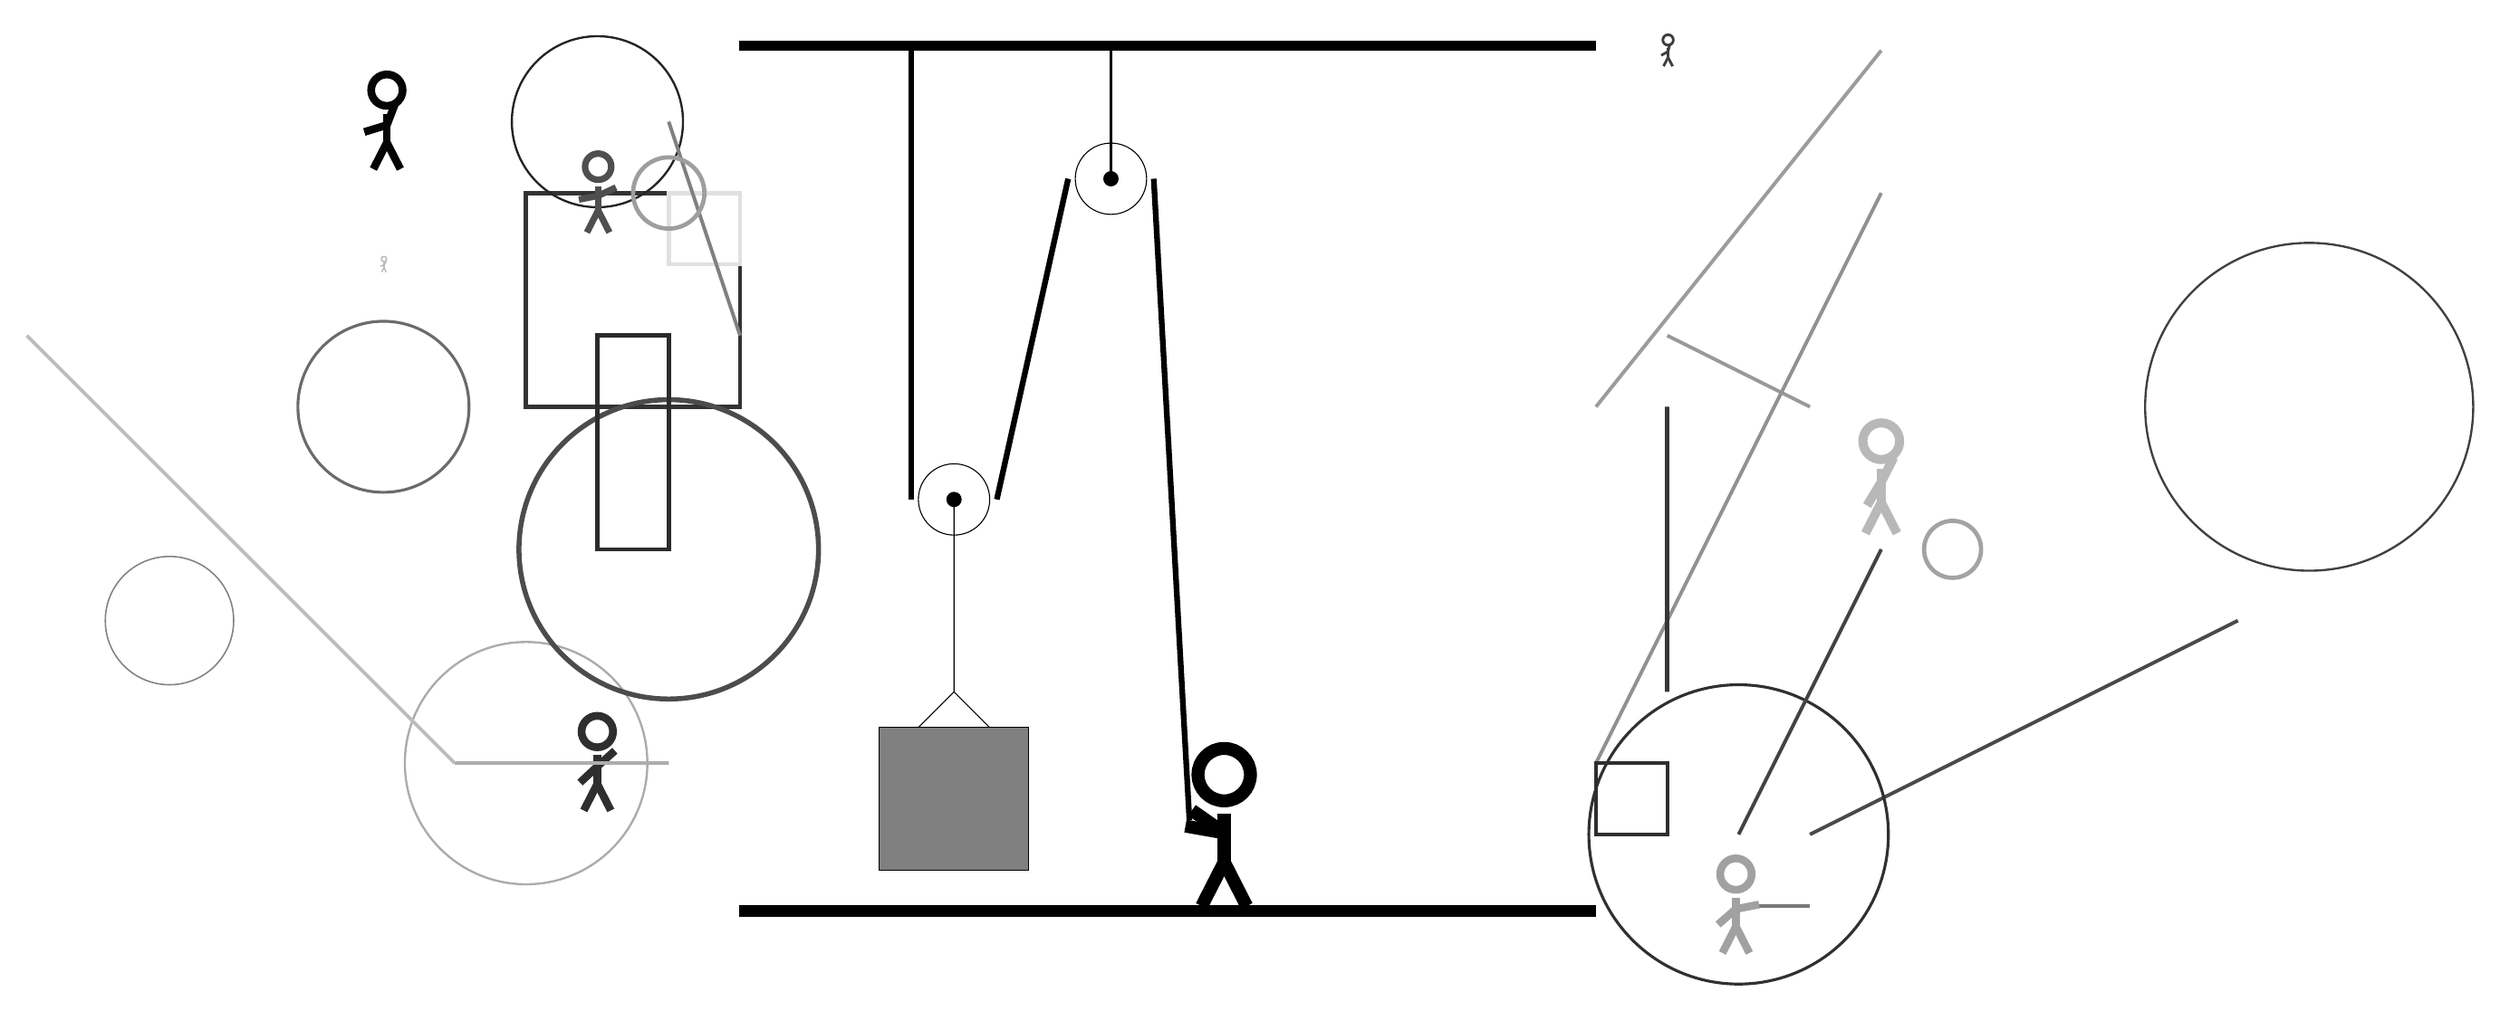
\begin{tikzpicture}
			%%%%% START %%%%%
			
			\draw[fill=black] (-2, 9) rectangle (10, 9.125);
			
			\draw (3.2, 7.2) circle (0.5);
			\draw[fill=black] (3.2, 7.2) circle (0.1);
			\draw[thick] (3.2, 7.2) -- (3.2, 9);
			
			\draw (1, 2.7) circle (0.5);
			\draw[fill=black] (1, 2.7) circle (0.1);
			
			\draw [line width=0.3mm, color=black!33](-5, -1) circle (1.7);
			
			\draw[line width=0.5mm, color=black!53](12, -3) -- (13, -3);
			\draw [line width=0.2mm, color=black!49](-10, 1) circle (0.9);
			\node[line width=0.7mm, color=black!76] at (11, 9) {\Strichmaxerl[2][29][77]};
			\draw[line width=0.5mm, color=black!71](13, -2) -- (19, 1);
			
			\draw[line width=0.6mm, color=black!80] (-2, 4) rectangle (-5, 7);
			\draw [line width=0.3mm, color=black!86](-4, 8) circle (1.2);
			\node[line width=0.2mm, color=black!28] at (14, 3) {\Strichmaxerl[7][59][63]};
			\node[line width=0.7mm, color=black!82] at (-4, -1) {\Strichmaxerl[6][43][42]};
			\draw[line width=0.5mm, color=black!40](13, 4) -- (11, 5);
			\draw [line width=0.7mm, color=black!70](-3, 2) circle (2.1);
			
			\draw[line width=0.6mm, color=black!83] (-4, 2) rectangle (-3, 5);
			\draw[line width=0.5mm, color=black!32] (-3, -1) rectangle (-6, -1);
			
			\draw [line width=0.4mm, color=black!58](-7, 4) circle (1.2);
			\node[line width=0.6mm, color=black!69] at (-4, 7) {\Strichmaxerl[5][11][25]};
			\draw [line width=0.3mm, color=black!73](13, -2) circle (0.0);
			
			\draw[line width=0.6mm, color=black!12] (-3, 6) rectangle (-2, 7);
			\draw[line width=0.5mm, color=black!43](10, -1) -- (14, 7);
			\node[line width=0.2mm, color=black!37] at (12, -3) {\Strichmaxerl[6][41][11]};
			\node[line width=0.4mm, color=black!98] at (-7, 8) {\Strichmaxerl[6][17][69]};
			\draw[line width=0.5mm, color=black!26](-6, -1) -- (-12, 5);
			
			\draw[line width=0.5mm, color=black!82] (11, -1) rectangle (10, -2);
			\draw[line width=0.5mm, color=black!39](14, 9) -- (10, 4);
			\draw[line width=0.7mm, color=black!79] (11, 4) rectangle (11, 0);
			\node[line width=0.2mm, color=black!28] at (-7, 6) {\Strichmaxerl[1][21][54]};
			
			\draw [line width=0.6mm, color=black!36](15, 2) circle (0.4);
			\draw[line width=0.5mm, color=black!50](-3, 8) -- (-2, 5);
			\draw [line width=0.4mm, color=black!81](12, -2) circle (2.1);
			\draw [line width=0.6mm, color=black!38](-3, 7) circle (0.5);
			\draw [line width=0.3mm, color=black!75](20, 4) circle (2.3);
			\draw[line width=0.5mm, color=black!74](12, -2) -- (14, 2);
			
			
			\draw (1, 2.7) -- (1, 0) -- (0.5, -0.5);
			\draw (1, 0) -- (1.5, -0.5);
			\draw[fill=black!50] (-0.05, -0.5) rectangle (2.05, -2.5);
			
			\draw[line width=0.8mm] (0.4, 9) -- (0.4, 2.7);
			\centerarc[line width=0.8mm](1, 2.7)(180:360:0.6);
			\draw[line width=0.8mm](1.6, 2.7) -- (2.6, 7.2);
			\centerarc[line width=0.8mm](3.2, 7.2)(0:180:0.6);
			\draw[line width=0.8mm](3.8, 7.2) -- (4.3, -1.8);
			
			\node at (4.7, -1.9) {\Strichmaxerl[10][-35][170]};
			
			\draw[fill=black] (-2, -3) rectangle (10, -3.15);
			
			%%%%% END %%%%%
		\end{tikzpicture}
	\end{figure}	
\end{document}